\documentclass{beamer}
\usepackage[utf8]{inputenc}

\usetheme{Madrid}
\usecolortheme{default}
\usepackage{amsmath,amssymb,amsfonts,amsthm}
\usepackage{txfonts}
\usepackage{tkz-euclide}
\usepackage{listings}
\usepackage{adjustbox}
\usepackage[T1]{fontenc}
\usepackage{array}
\usepackage{tabularx}
\usepackage{gvv}
\usepackage{lmodern}
\usepackage{circuitikz}
\usepackage{tikz}
\usepackage{graphicx}

\setbeamertemplate{page number in head/foot}[totalframenumber]

\usepackage{tcolorbox}
\tcbuselibrary{minted,breakable,xparse,skins}



\definecolor{bg}{gray}{0.95}
\DeclareTCBListing{mintedbox}{O{}m!O{}}{%
  breakable=true,
  listing engine=minted,
  listing only,
  minted language=#2,
  minted style=default,
  minted options={%
    linenos,
    gobble=0,
    breaklines=true,
    breakafter=,,
    fontsize=\small,
    numbersep=8pt,
    #1},
  boxsep=0pt,
  left skip=0pt,
  right skip=0pt,
  left=25pt,
  right=0pt,
  top=3pt,
  bottom=3pt,
  arc=5pt,
  leftrule=0pt,
  rightrule=0pt,
  bottomrule=2pt,
  toprule=2pt,
  colback=bg,
  colframe=orange!70,
  enhanced,
  overlay={%
    \begin{tcbclipinterior}
    \fill[orange!20!white] (frame.south west) rectangle ([xshift=20pt]frame.north west);
    \end{tcbclipinterior}},
  #3,
}
\lstset{
    language=C,
    basicstyle=\ttfamily\small,
    keywordstyle=\color{blue},
    stringstyle=\color{orange},
    commentstyle=\color{green!60!black},
    numbers=left,
    numberstyle=\tiny\color{gray},
    breaklines=true,
    showstringspaces=false,
}
%------------------------------------------------------------
%This block of code defines the information to appear in the
%Title page
\title %optional
{ 4.8.14}

%\subtitle{A short story}

\author % (optional)
{Hemanth Reddy-AI25BTECH11018}



\begin{document}


\frame{\titlepage}
\begin{frame}{Question}

Let $\vec{P} (3,2,6)$ be a point in space and $\vec{Q}$ be a point on the line
$ \vec{r} = (\hat{i} - \hat{j} + 2\hat{k}) + \mu(-3\hat{i} + \hat{j} + 5\hat{k}). $
Then the value of $\mu$ for which the vector $\overrightarrow{PQ}$ is parallel to the plane $x - 4y + 3z = 1$ is 
\end{frame}



\begin{frame}{Theoretical Solution}
\textbf{Solution:}\\


\begin{align}
   \text{ The position vector of point }  \vec{P} \text{ is }
 \myvec{ 3 \\ 2\\ 6 } 
\end{align}

Point $\vec{Q}$ lies on line $\vec{r}$ .So

\begin{align}
   \text{ The position vector of point }  \vec{Q} \text{ is }
 \myvec{ 1-3\mu\\ -1+\mu \\ 2+5\mu } 
\end{align}

\begin{align}
    \overrightarrow{PQ} = \vec{Q} -\vec{P} = \myvec{ 1-3\mu-3\\ -1+\mu -2\\ 2+5\mu -6} = \myvec{ -2-3\mu\\ -3+\mu \\ -4+5\mu } 
\end{align}

\end{frame}

\begin{frame}{Theoretical Solution}

Equation of plane is $x - 4y + 3z = 1$ 
\begin{align}
    \text{ Normal of plane is} \quad \vec{n} =\myvec{ 1 \\ -4\\ 3 } 
\end{align}

$\overrightarrow{PQ}$ is parallel to the plane ,So $\vec{n}^{T}(\vec{PQ})=0$

\begin{align}
   \vec{n}^{T}(\vec{PQ})= \myvec{ 1 & -4 & 3 } \myvec{ -2-3\mu\\ -3+\mu \\ -4+5\mu } =0
\end{align}

\begin{align}
    -2-3\mu+12-4\mu-12+15\mu=0\\
    -2+8\mu=0\\
    \mu=\frac{1}{4}
\end{align}

\end{frame}

\begin{frame}[fragile]
    \frametitle{C Code}
    \begin{lstlisting}

#include <stdio.h>

// This function calculates the value of mu
double solve_mu() {
    // Coordinates of point P(3, 2, 6)
    double px = 3.0;
    double py = 2.0;
    double pz = 6.0;

    // Components of the starting point of the line: (1, -1, 2)
    double rx = 1.0;
    double ry = -1.0;
    double rz = 2.0;

    // Components of the direction vector of the line: (-3, 1, 5)
    double vx = -3.0;
    double vy = 1.0;
    double vz = 5.0;

   

    \end{lstlisting}
\end{frame}

\begin{frame}[fragile]
    \frametitle{C Code}
    \begin{lstlisting}

 // Normal vector components of the plane: (1, -4, 3)
    double nx = 1.0;
    double ny = -4.0;
    double nz = 3.0;

    // The vector PQ is calculated as Q - P, where Q = r + mu*v
    // PQ = ( (rx + mu*vx) - px, (ry + mu*vy) - py, (rz + mu*vz) - pz )
    // PQ = ( (1 + mu*(-3)) - 3, (-1 + mu*1) - 2, (2 + mu*5) - 6 )
    // PQ = ( -2 - 3*mu, -3 + mu, -4 + 5*mu )

    // The condition for PQ to be parallel to the plane is that its dot product
    // with the plane's normal vector n is zero.
    // PQ . n = 0
    // (-2 - 3*mu)*nx + (-3 + mu)*ny + (-4 + 5*mu)*nz = 0
    
   

    \end{lstlisting}
\end{frame}

\begin{frame}[fragile]
    \frametitle{C Code}
    \begin{lstlisting}

 // ((-2 - 3*mu)*1) + ((-3 + mu)*-4) + ((-4 + 5*mu)*3) = 0
    // -2 - 3*mu + 12 - 4*mu - 12 + 15*mu = 0
    // Collect mu terms: (-3 - 4 + 15)*mu = 8*mu
    // Collect constant terms: -2 + 12 - 12 = -2
    // So, 8*mu - 2 = 0
    // 8*mu = 2
    // mu = 2 / 8
    
    // The coefficients of the linear equation for mu: A*mu + B = 0
    // A = vx*nx + vy*ny + vz*nz - (dot product of direction vector with normal vector)
    double A = vx * nx + vy * ny + vz * nz;
    
    // B = (rx - px)*nx + (ry - py)*ny + (rz - pz)*nz - (dot product of position vector PQ with normal vector)
    double B = (rx - px) * nx + (ry - py) * ny + (rz - pz) * nz;



    \end{lstlisting}
\end{frame}

\begin{frame}[fragile]
    \frametitle{C Code}
    \begin{lstlisting}


    // Solve for mu
    double mu = -B / A;
    
    return mu;
}

int main() {
    double result = solve_mu();
    printf("The value of mu is: %f\n", result);
    return 0;
}

    \end{lstlisting}
\end{frame}

\begin{frame}[fragile]
    \frametitle{Python Code}
    \begin{lstlisting}

import numpy as np
import matplotlib.pyplot as plt
from mpl_toolkits.mplot3d import Axes3D
from matplotlib.patches import Rectangle # For proxy artist in legend

def plot_3d_solution_refined():
    # --- 1. Given Data ---
    # Point P(3, 2, 6)
    P = np.array([3, 2, 6])

    # Line r = (i - j + 2k) + mu(-3i + j + 5k)
    line_base = np.array([1, -1, 2])
    line_direction = np.array([-3, 1, 5])

    # Plane: x - 4y + 3z = 1
    plane_normal = np.array([1, -4, 3])
    plane_d = 1 # Constant term in ax+by+cz=d

 

    \end{lstlisting}
\end{frame}

\begin{frame}[fragile]
    \frametitle{Python Code}
    \begin{lstlisting}

   # --- 2. Calculate mu ---
    base_minus_P = line_base - P
    dot_product_base_P_normal = np.dot(base_minus_P, plane_normal)
    dot_product_direction_normal = np.dot(line_direction, plane_normal)

    if dot_product_direction_normal == 0:
        if dot_product_base_P_normal == 0:
            print("The line lies on the plane or is parallel to it.")
        else:
            print("The line is parallel to the plane, but PQ can never be parallel to the plane.")
        return

   

    \end{lstlisting}
\end{frame}

\begin{frame}[fragile]
    \frametitle{Python Code}
    \begin{lstlisting}

 mu = -dot_product_base_P_normal / dot_product_direction_normal
    print(f"Calculated value of mu: {mu}")

    # --- 3. Calculate Q and PQ vector for the specific mu ---
    Q = line_base + mu * line_direction
    vector_PQ = Q - P
    print(f"Point Q for mu={mu:.2f}: {Q}")
    print(f"Vector PQ: {vector_PQ}")
    print(f"Dot product of PQ and plane normal (should be ~0): {np.dot(vector_PQ, plane_normal):.4e}")


    # --- 4. 3D Plotting ---
    fig = plt.figure(figsize=(12, 10))
    ax = fig.add_subplot(111, projection='3d')

    

    \end{lstlisting}
\end{frame}


\begin{frame}[fragile]
    \frametitle{Python Code}
    \begin{lstlisting}

# Plot point P
    ax.scatter(P[0], P[1], P[2], color='green', s=150, edgecolors='black', label='Point P (3,2,6)')

    # Plot the line Q is on
    t_line = np.linspace(-3, 3, 100) # Reduced range for the line for better focus
    line_x = line_base[0] + t_line * line_direction[0]
    line_y = line_base[1] + t_line * line_direction[1]
    line_z = line_base[2] + t_line * line_direction[2]
    ax.plot(line_x, line_y, line_z, color='purple', linewidth=2, label='Line r (Q is on this)')

    # Plot point Q for the calculated mu
    ax.scatter(Q[0], Q[1], Q[2], color='red', s=150, edgecolors='black', label=fr'Point Q for $\mu={mu:.2f}$')

  

    \end{lstlisting}
\end{frame}


\begin{frame}[fragile]
    \frametitle{Python Code}
    \begin{lstlisting}

  # Plot vector PQ
    ax.quiver(P[0], P[1], P[2],
              vector_PQ[0], vector_PQ[1], vector_PQ[2],
              color='blue', linewidth=3, arrow_length_ratio=0.15, label='Vector PQ')

    # --- Plot the plane x - 4y + 3z = 1 ---
    # Define a bounding box for the plane around P and Q
    # Get the min/max of P and Q coords to set plane range
    all_x = np.array([P[0], Q[0], line_base[0]])
    all_y = np.array([P[1], Q[1], line_base[1]])
    all_z = np.array([P[2], Q[2], line_base[2]])

    x_min, x_max = np.min(all_x) - 2, np.max(all_x) + 2
    y_min, y_max = np.min(all_y) - 2, np.max(all_y) + 2

    xx, yy = np.meshgrid(np.linspace(x_min, x_max, 20),
                         np.linspace(y_min, y_max, 20))
    
   

    \end{lstlisting}
\end{frame}

\begin{frame}[fragile]
    \frametitle{Python Code}
    \begin{lstlisting}

 # Solve for z: z = (d - Ax - By) / C
    # Ensure C is not zero to avoid division by zero
    if plane_normal[2] != 0:
        zz = (plane_d - plane_normal[0]*xx - plane_normal[1]*yy) / plane_normal[2]
    else: # If normal_z is 0, the plane is vertical, plot by fixing one variable
        # This case is not relevant for x-4y+3z=1 but good for robustness
        print("Warning: Plane has no Z component in normal, adjusting plot method.")
        # Need a more complex way to plot vertical planes if this happens

    ax.plot_surface(xx, yy, zz, alpha=0.6, color='cyan', label='Plane') # Increased alpha for visibility

   

    \end{lstlisting}
\end{frame}

\begin{frame}[fragile]
    \frametitle{Python Code}
    \begin{lstlisting}

 # Create a proxy artist for the plane's legend entry
    plane_proxy = Rectangle((0, 0), 1, 1, fc='cyan', alpha=0.6)
    
    # Plot the normal vector of the plane (from a point on the plane for clarity)
    # Let's start the normal vector from Q for better context to PQ
    ax.quiver(Q[0], Q[1], Q[2], # Start point (Q)
              plane_normal[0], plane_normal[1], plane_normal[2], # Direction components
              color='orange', linewidth=2, length=np.linalg.norm(plane_normal)*0.8, arrow_length_ratio=0.2, label='Plane Normal')


    ax.set_xlabel('X axis')
    ax.set_ylabel('Y axis')
    ax.set_zlabel('Z axis')
   

    \end{lstlisting}
\end{frame}

\begin{frame}[fragile]
    \frametitle{Python Code}
    \begin{lstlisting}

 ax.set_title(fr'3D Visualization: Vector PQ Parallel to Plane (for $\mu={mu:.2f}$)')
    
    
    # Use explicit handles and labels for the legend for better control
    handles = [
        plt.Line2D([0], [0], marker='o', color='w', markerfacecolor='green', markersize=10, label='Point P (3,2,6)'),
        plt.Line2D([0], [0], color='purple', lw=2, label='Line r'),
        plt.Line2D([0], [0], marker='o', color='w', markerfacecolor='red', markersize=10, label=fr'Point Q for $\mu={mu:.2f}$'),
        plt.Line2D([0], [0], color='blue', lw=3, label='Vector PQ'),
       

    \end{lstlisting}
\end{frame}

\begin{frame}[fragile]
    \frametitle{Python Code}
    \begin{lstlisting}

 plane_proxy, # The proxy artist for the plane
        plt.Line2D([0], [0], color='orange', lw=2, label='Plane Normal Vector')
    ]
    labels = [h.get_label() for h in handles]
    ax.legend(handles, labels, loc='best', fontsize='small')
    
    # Set axis limits based on data
    ax.set_xlim(np.min(all_x)-3, np.max(all_x)+3)
    ax.set_ylim(np.min(all_y)-3, np.max(all_y)+3)
    ax.set_zlim(np.min(all_z)-3, np.max(all_z)+3)
    
    # Set equal aspect ratio for a more accurate visual representation (optional, can sometimes distort view)
    # ax.set_box_aspect([1,1,1]) # This requires all three limits to be set symmetrically or specified
    


    \end{lstlisting}
\end{frame}

\begin{frame}[fragile]
    \frametitle{Python Code}
    \begin{lstlisting}

    # Adjust view angle for better perspective
    ax.view_init(elev=20, azim=-120) # Changed azim for a different view

    plt.tight_layout()
    plt.show()

# Run the plotting function
plot_3d_solution_refined()

    \end{lstlisting}
\end{frame}

\begin{frame}{Plot}

\begin{figure}
    \centering
    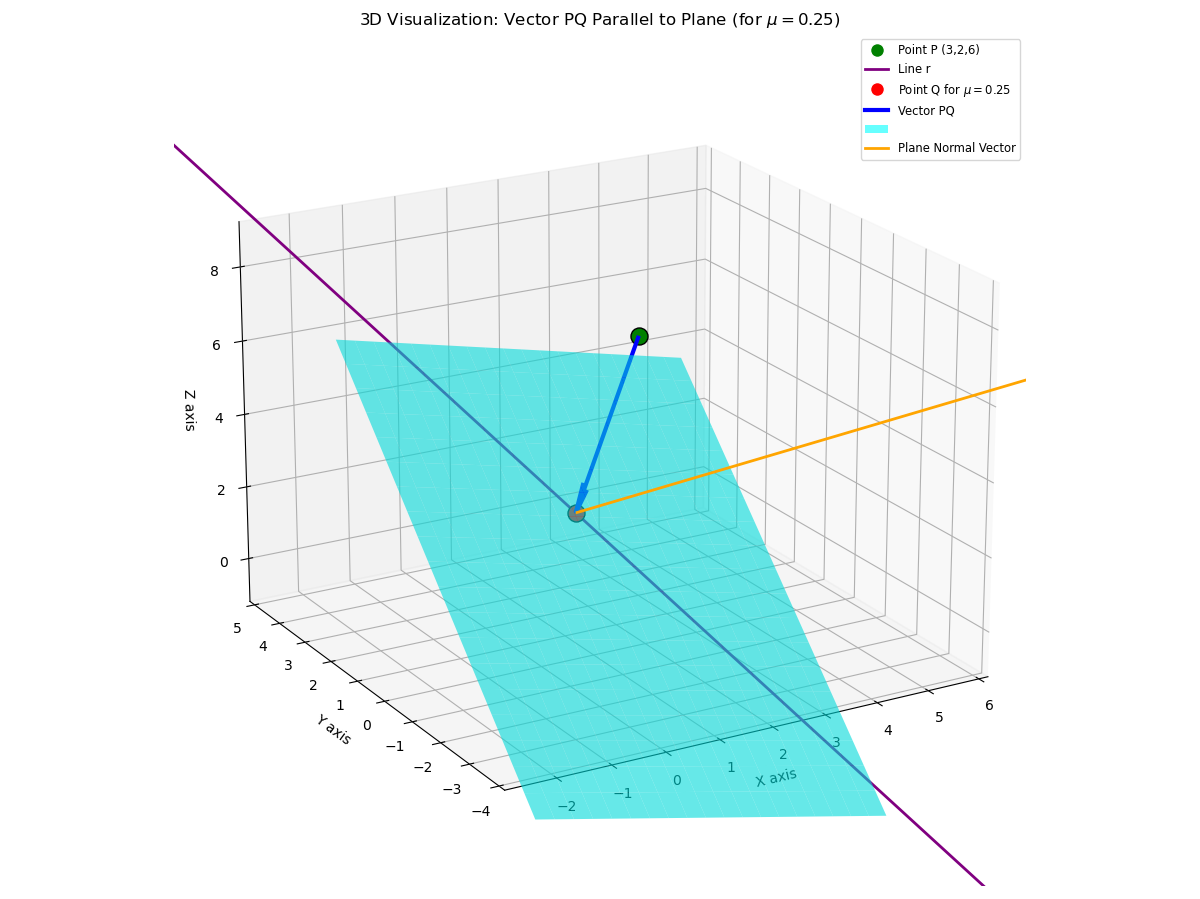
\includegraphics[width=0.8\linewidth]{Beamer/figs/Plane1.png}
    \caption{}
    \label{fig:placeholder}
\end{figure}

\end{frame}

\end{document}





